
\section{Test}


\begin{frame}[fragile]{Test Slide with styles}
\begin{itemize}
\item Bullet \index{Bullet} item 0 $\tikzmarkin<1>{a1}a_i\tikzmarkend{a1} + b_j = 10 $
\item Bullet \index{Bullet} item 2 with code\footnote{Do you like footnotes?}
\begin{minted}[mathescape]{python}
    # footnotesize
    for  a in range(10):
    !  \tikzmarkin<1->{b}yield a\tkizmarkend{b}
    # $\xmapsto[encode]{utf-8}$
    # $a \rightarrow b^{c}$
    |\index{return}return| False
\end{minted}
\item Bullet Item 3 \pdfmarkupcomment[markup=Underline,color=black,author=Foo]{$a_i$}{Comment} $ + b_j = 10 $
\end{itemize}
\end{frame}

\begin{frame}[fragile]{Test Slide with styles}
\begin{enumerate}
\item Enumerate1 \index{enumerate} \pdfcomment{Pdf Comment Test Slide with styles}
    \begin{enumerate}
    \item EnumerateA  \pyver{w\"urstel re}sults
    \item \texttt{Inline minted ipython}
    \item Una linea \pdfmarkupcomment[markup=Underline,color=black,author=Gumbo]{Altro commento  \#}{This is the injected part of a SQL injection}
    \item w\"urstelstra\ss e
    \end{enumerate}

\item Enumerate2 \`{e} 
 [\red{196}, \blue{168}] 
\begin{pythoncode*}{escapeinside=||}
@|\pyver{decorator}|
def foo(tmp):
    def bar(*args):
        |\index{return}return| tmp(|$*args_{i}$|)
    |\index{return}return| bar
\end{pythoncode*}

\end{enumerate}

\end{frame}

\begin{frame}[fragile]{Tabular and image}
A Tabular follows \\
\begin{tabular}{|c|c|}\hline
Cell 1 & Cell 2 \\
\hline 
\end{tabular}
\\
\begin{table}
\begin{tabular}{|c|c|}\hline
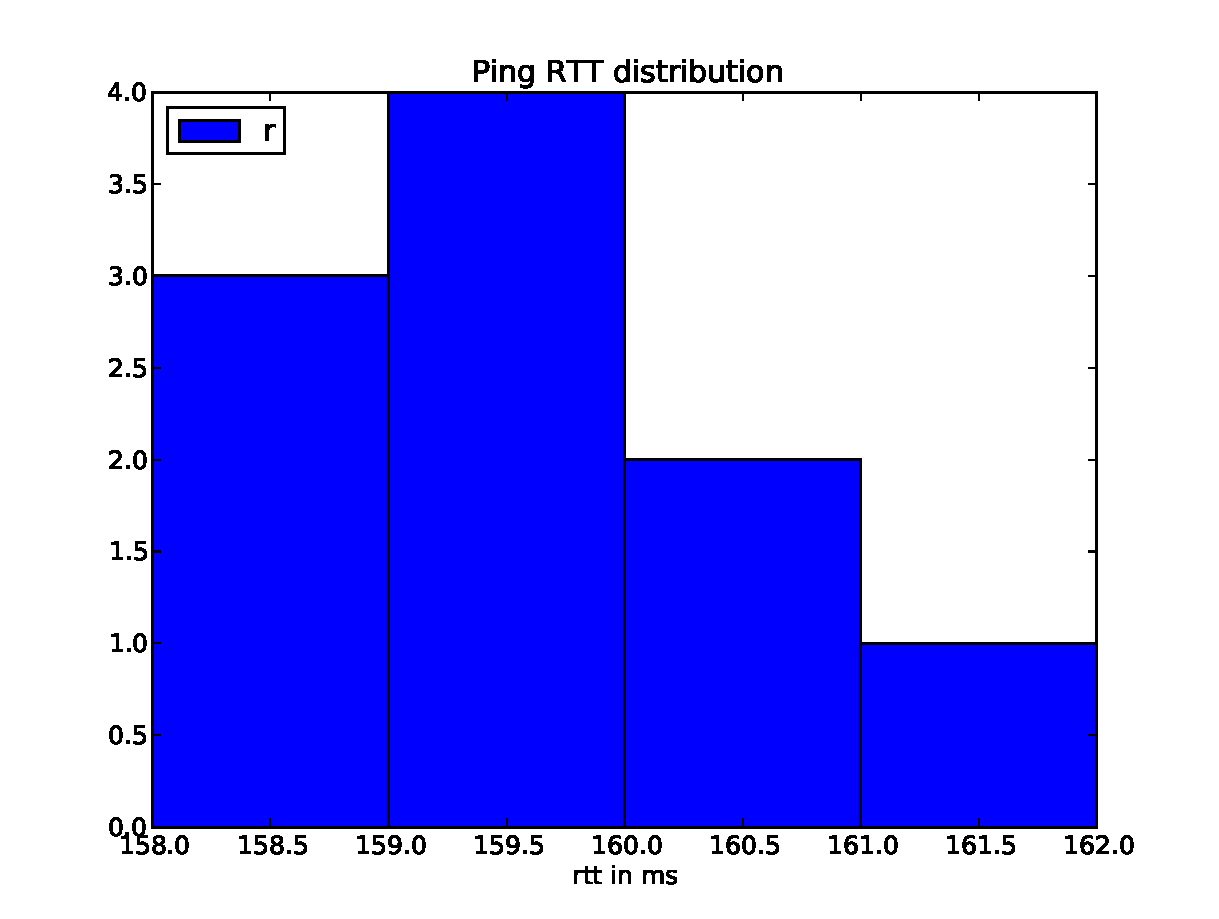
\includegraphics[height=4cm]{ping_distribution.pdf}   & 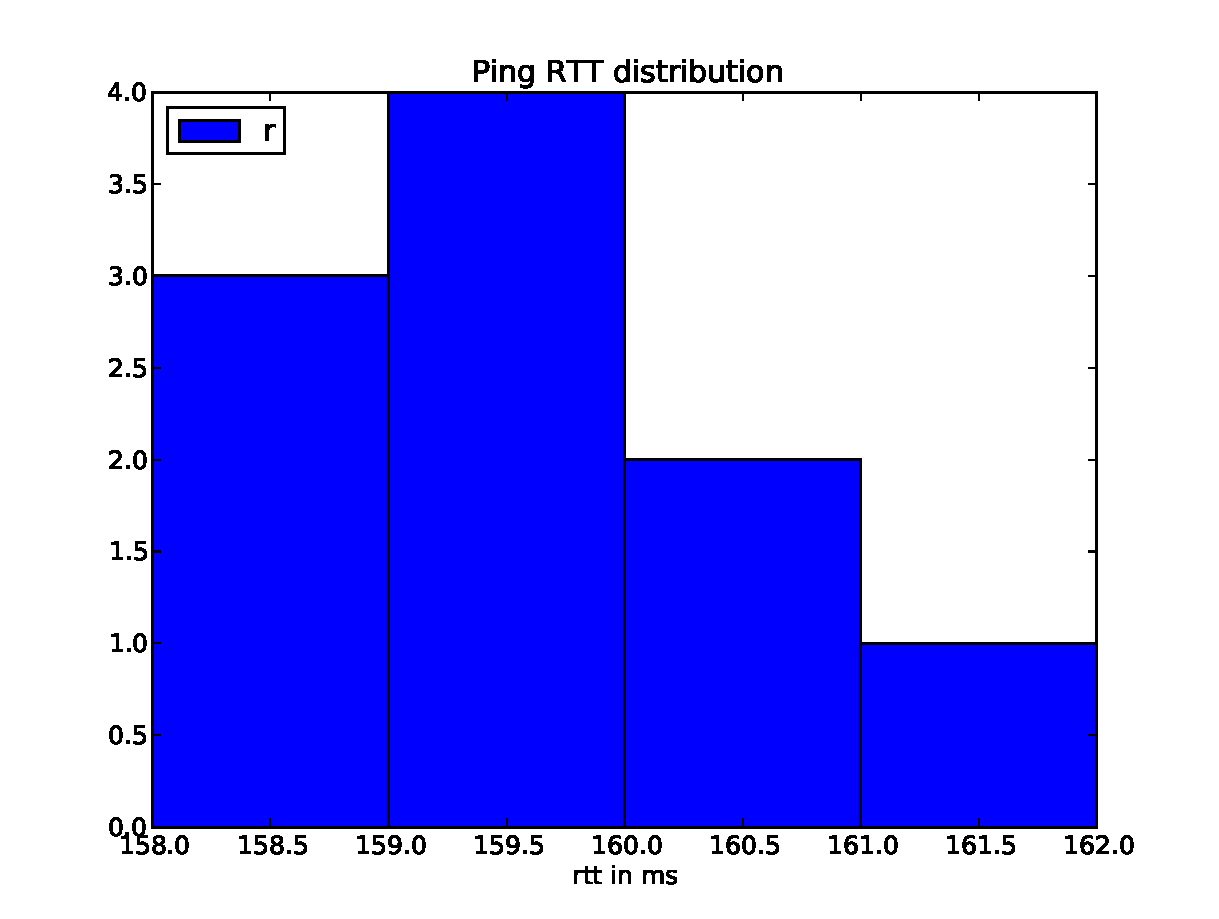
\includegraphics[height=4cm]{ping_distribution.pdf}  \\
\hline 
\end{tabular}
\end{table}
\end{frame}

\begin{frame}[fragile]{Simple Column}
\begin{columns}
\column[t]{5cm}
\begin{pythoncode}
"""using set and dict
"""
distro = {x: rtt.count(x) 
  for x in set(rtt)}
# or using a
from collections import defaultdict
distro = defaultdict(int)
for x in rtt:
    distro[x] += 1
    

\end{pythoncode}
\column[t]{5cm}
-skip-\\
-skip-\\
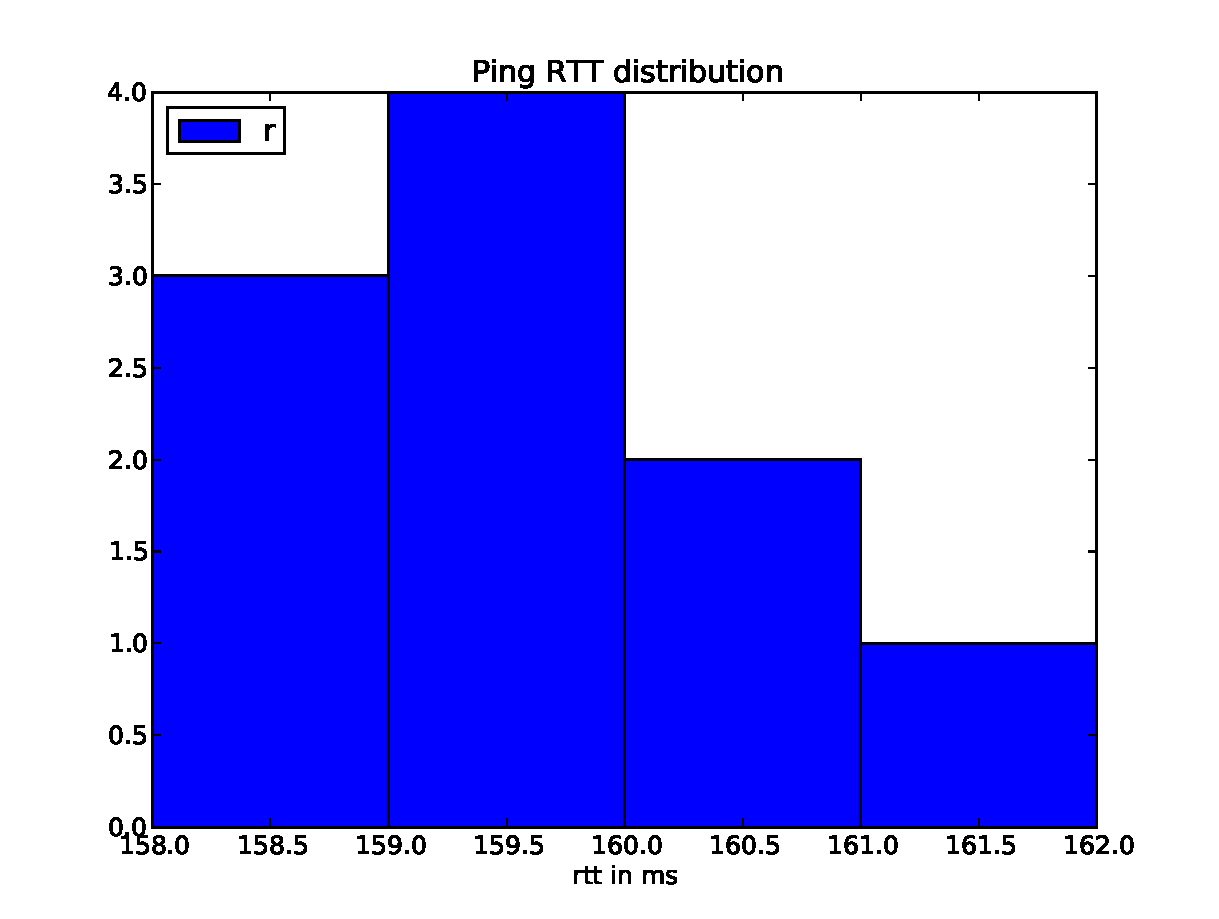
\includegraphics[height=4cm]{ping_distribution.pdf}  
\end{columns}
\end{frame}


\begin{frame}[fragile]{2-columns and verbatim}
Two columns
\begin{columns}

\column[t]{5cm}
1
2
3
\begin{verbatim}
4
5
6
\end{verbatim}

\column[t]{5cm}
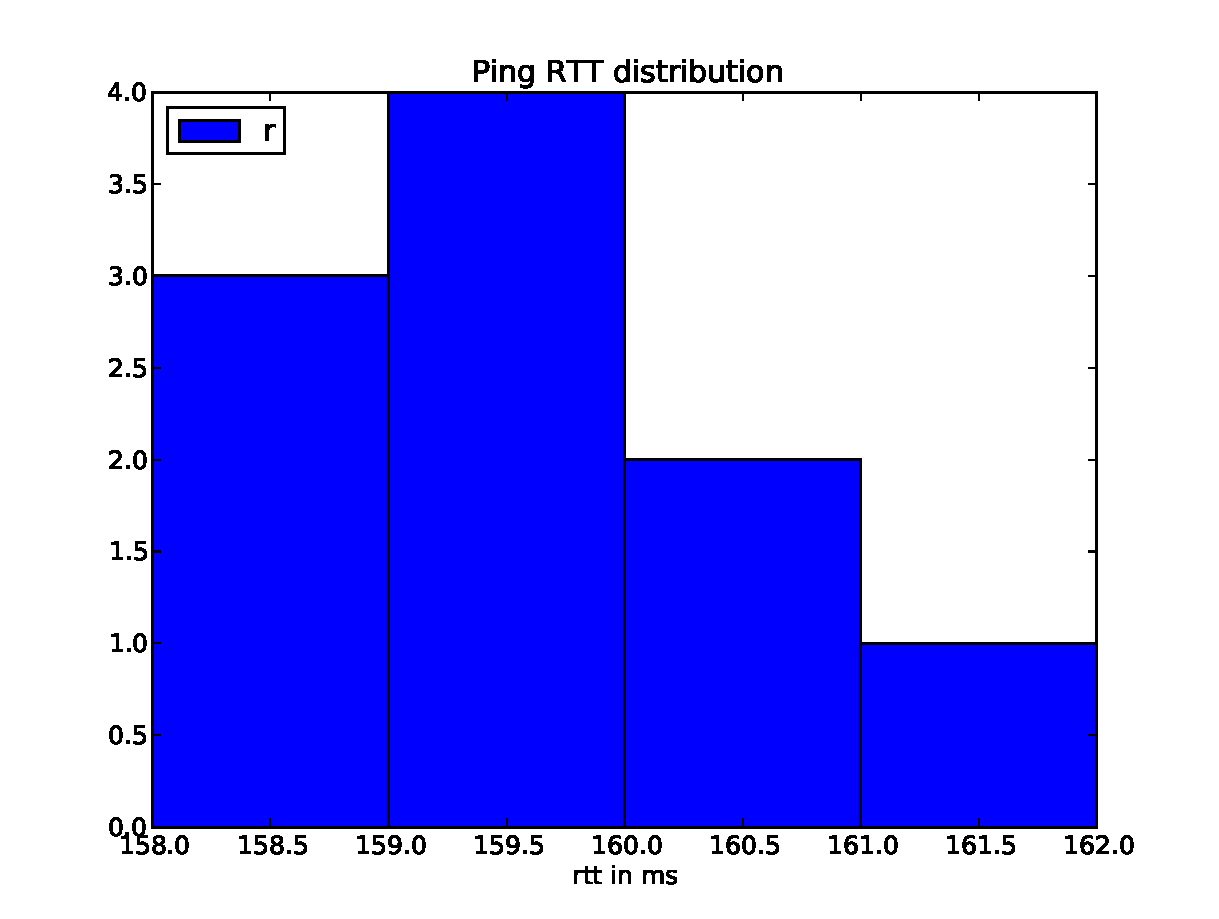
\includegraphics[height=4cm]{ping_distribution.pdf}  
\end{columns}

\end{frame}



\begin{frame}[fragile]{Simple processing: distribution}
\begin{columns}
\column[t]{5cm}
\begin{pythoncode}
"""using set and dict
"""
distro = {x: rtt.count(x) 
  for x in set(rtt)}
# or using a
from collections import defaultdict
distro = defaultdict(int)
for x in rtt:
    distro[x] += 1
    
a
a
a
a
a
a
a
a
a

    
    
    
    
\end{pythoncode}
\column[t]{5cm}
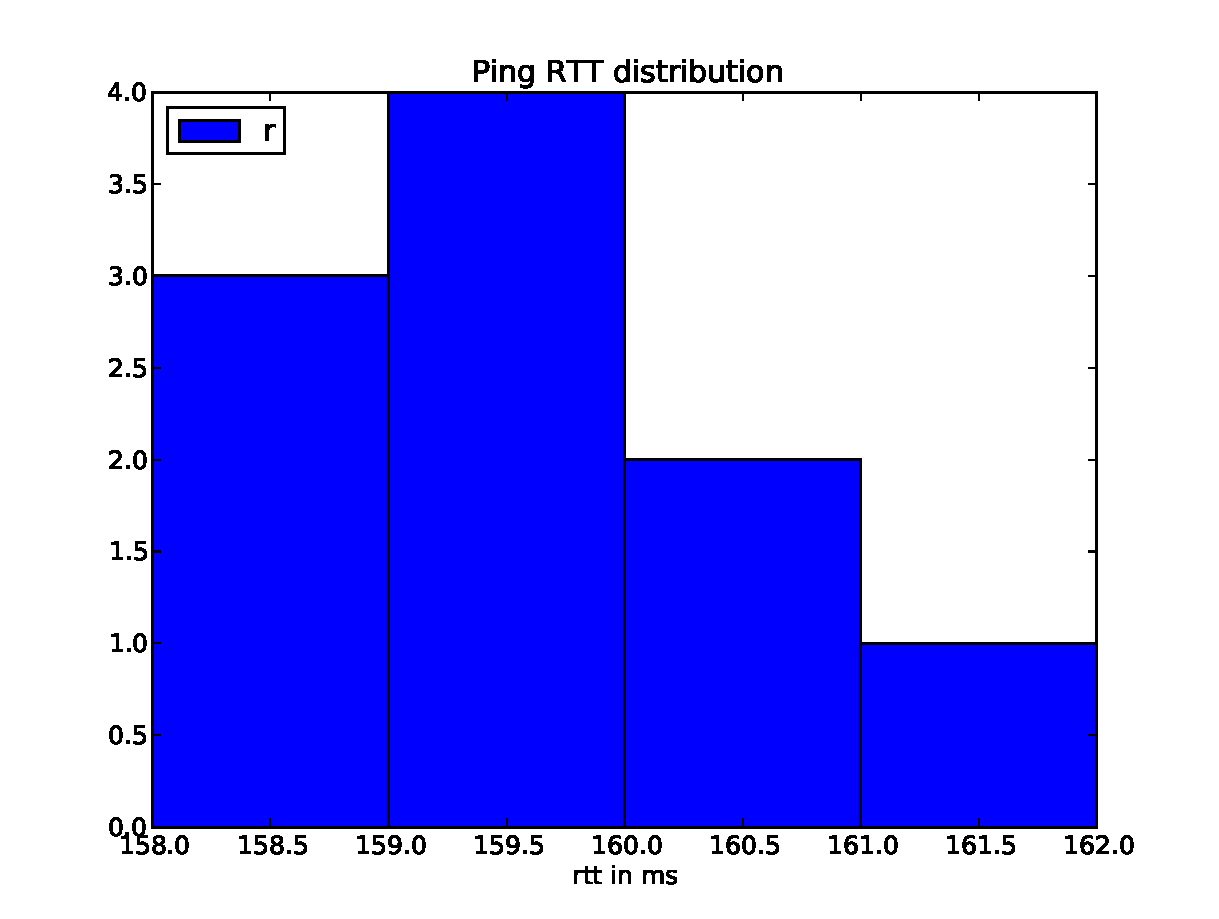
\includegraphics[width=4cm]{ping_distribution.pdf}  
\end{columns}
%Homework: which is faster?
\end{frame}

\begin{frame}{Index}
\printindex

fooo bar

\end{frame}
